\section{Experimental Framework}

To illustrate our theoretical results, we evaluate the ability of the models to capture homophily and the preferential attachment effect on artificial and real networks. In this section, we beforehand present our measures for both properties. Afterwards, we describe the datasets that we have used, then we will explain our evaluation protocol. Finally we present our results and their relations to the theoretic framework.

\subsection{Measures for the Properties}

\textit{Homophily Indicators}

To evaluate homophily in a given attributed network, we use the measures introduced by \cite{largeron2015}, adapted from the test proposed by \cite{Easley2010}.  This test compares an expected homophily measure corresponding to the probability for two vertices to be similar with an observed homophily measure defined as the probability that two linked vertices are similar. More precisely, given a contingency table defined as follows:

$a = Card\{(i,j)\in V\times (V-1) / (i,j) \in E \land s(i,j)\}$\\
$b = Card\{(i,j)\in V\times (V-1) / (i,j) \in E \land \neg{s(i,j)}\}$\\ 
$c = Card\{(i,j)\in V\times (V-1) / (i,j) \notin E \land s(i,j)\}$\\
$d = Card\{(i,j)\in V\times (V-1) / (i,j) \notin E \land \neg{s(i,j)}\}$\\
%$\frac{N*(N-1)}{2}$ is the total count of  the cells in the contingency table.\\

where  s(i,j) indicates that i and j are considered as similar, observed homophily, denoted $H_{obs}$, is given by $\frac{a}{a+b}$.\\
This measure  is equal to 1 when all the pairs of linked vertices are similar. Consequently, high values suggest an homophily effect.

Moreover, $H_{obs}$ can be compared with an expected measure, $H_{expec}$, defined by  $ \frac{a+c}{a+b+c+d}$.\\

If the expected measure is significantly less than the observed measure, then there is evidence for homophily.\\

\textit{Preferential attachment}

Preferential attachment leads to networks characterized by a degree distribution with heavy tail which can take the form of a power law. To evaluate this property, we  plot the degree distributions in log log scale for the original network and the generated network. Comparaison of the degree distribution with a straight line gives us a qualitative measure for the preferential attachment.\\

\subsection{Datasets}
To demonstrate the potential of the models to generate graphs verifying properties occurring in original networks, we consider four artificial networks and two real networks.\\

\textit{Artificial networks}

The artificial networks have been generated with ANC-Generator \cite{largeron2015}. This generator has been chosen because it allows to build attributed graphs with community structure faithfully following the known properties of real-world networks such as preferential attachment and homophily. 
\textbf{ ARV peut on faire le lien ici entre les facteurs latents et les attributs - communautés ? }.
Moreover, by modifying the parameters, these properties can be weakened. Finally, ANC-Generator is available under the terms of the GNU Public Licence and the parameters can be shared for experiments reproducibility. 

Four artificial networks have been generated, each one corresponding to a configuration  regarding the properties of interest.
Both properties are verified in the first one ($Network1$) whereas none of them is checked in the $Network4$.  There is only an evidence for homophily in the network $Network2$ and  preferential attachment in the network  $Network3$. Table 1 summarizes these four configurations. \\ 

\textbf{Ajouter parametrage}  

% \textit{Real networks}
\textit{Real networks}

We evaluate also the models on two  real networks.
The first one \footnote{available at:} is built from an online community of 1899 students from the University of California. Each node corresponds to a user and a directed edge represents a sent message. 
The second one \footnote{available at:} is an internal email communication network between employees of a mid-sized manufacturing company. Each vertex is associated to an employee and an oriented link represents like previously a sent email.

Table 1 summarizes basic characteristics of these synthetic and real datasets \textbf{ Mettre nombre de sommets, de liens}.

\subsection{Evaluation Protocol}
For each datasets described,  we run a MCMC inference consisting of 200 iterations to learn the posterior distribution of each the IMMSB model and ILFM, described in \ref{sec:models}. For IMMSB concentration parameters of HDP were optimized following \cite{HDP} using vague gamma prior $\alpha_0 \sim \text{Gamma}(1,1)$ and $\gamma \sim \text{Gamma}(1,1)$. Parameters for the matrix weights were fixed to $\lambda_0=\lambda_1=0.1$. For ILFM, the IBP hyper-parameters were fixed to $\alpha=0.5$ weights hyper-parameters to $\sigma_w = 1$.

Our evaluation rely then in two strategy:

%We track how well the models can reproduce the properties on the generated networks. In this view, using the same indicators, we compare the values computed respectively on the original network and on the generated network.


\subsubsection{Predictive performance}
For all our experiments, we separate our datasets into a training set representing 80 \% of the size of the network, and 20\% for a testing set, randomly chosen. Inference is then run over 200 iterations. 

We performed a predictive analysis on the testing set and compared the performance prediction of each models with the property of networks. 
The predictive performance of models is calculated using a traditional precision and recall for the links predicted.\\
Equation precision rappel ?

\subsubsection{Generative network}
We used the relational models as generative process and generate a \emph{generative} network. We then verify that the properties of interest are well satisfied on this synthetic network.


\subsection{Results}
The table \ref{table:immsb} show the predictive performance in term of overall precision for IMMSB for different size of class learned. Firstly, it is interesting to see that IMMSB perform better in all cases when the networks are bursty. Secondly, it's worth to note that the models has a tendency to perform better when the homophily is not strongly present. This can be explain by the fact that IMMSB allows relation between classes, and because strong homophily will conduct to more dense community in a network.


\begin{table} \label{table:immsb}
\begin{tabular}{lrrrr}
\hline                                                                             
 immsb / mask all   &        5 &       10 &       15 &       20 \\                 
\hline                                                                             
 Graph7 b/h         & 0.989636 & 0.989939 & 0.990358 & 0.989873 \\                 
 Graph12 b/-h       & 0.99179  & 0.991689 & 0.991997 & 0.992259 \\                 
 Graph4 -b/h        & 0.886844 & 0.888035 & 0.908348 & 0.906659 \\                 
 Graph10 -b/-h      & 0.979057 & 0.979144 & 0.979487 & 0.979366 \\                 
\hline                                                                             
\end{tabular}  
    \caption{IMMSB prediction performance result on synthetic networks, for different size of classes infered.}
\end{table}


The table \ref{table:ibp} shows the precision and recall results, for each networks. Additionally we show the number of latent features to which ILFM has converged. We can see that ILFM is significantly better than IMMSB at predicting over homophilic network, with a small number of features. Besides, although ILFM can achieve good results, for bursty network, we see that the models learn more features for non-bursty networks compared to IMMSB. 

\begin{table} \label{table:ibp}
\begin{tabular}{lrrrr}
\hline
 ibp / mask all   &     global &   precision &      rappel &   K-\ensuremath{>} \\
\hline
 Graph7 b/h       & nan        & nan         & nan         &   nan \\
 Graph12 b/-h     &   0.992204 &   0.0532044 &   0.0537897 &    13 \\
 Graph4 -b/h      &   0.939498 &   0.496967  &   0.490113  &    10 \\
 Graph10 -b/-h    &   0.981577 &   0.0910384 &   0.09826   &    11 \\
\hline
\end{tabular}  
    \caption{ILFM predictive performance result on synthetic networks}
\end{table}

Our results confirm the theoretical analysis on nonparametric models, concerning their affinity to the preferential attachment effect and the homophily effect.

%Our experiments evaluate the preferential attachment and the local preferential attachment on the learned communities trough respectively the distribution of degrees in the networks and inside the communities.
\begin{figure}[h]
	\centering
	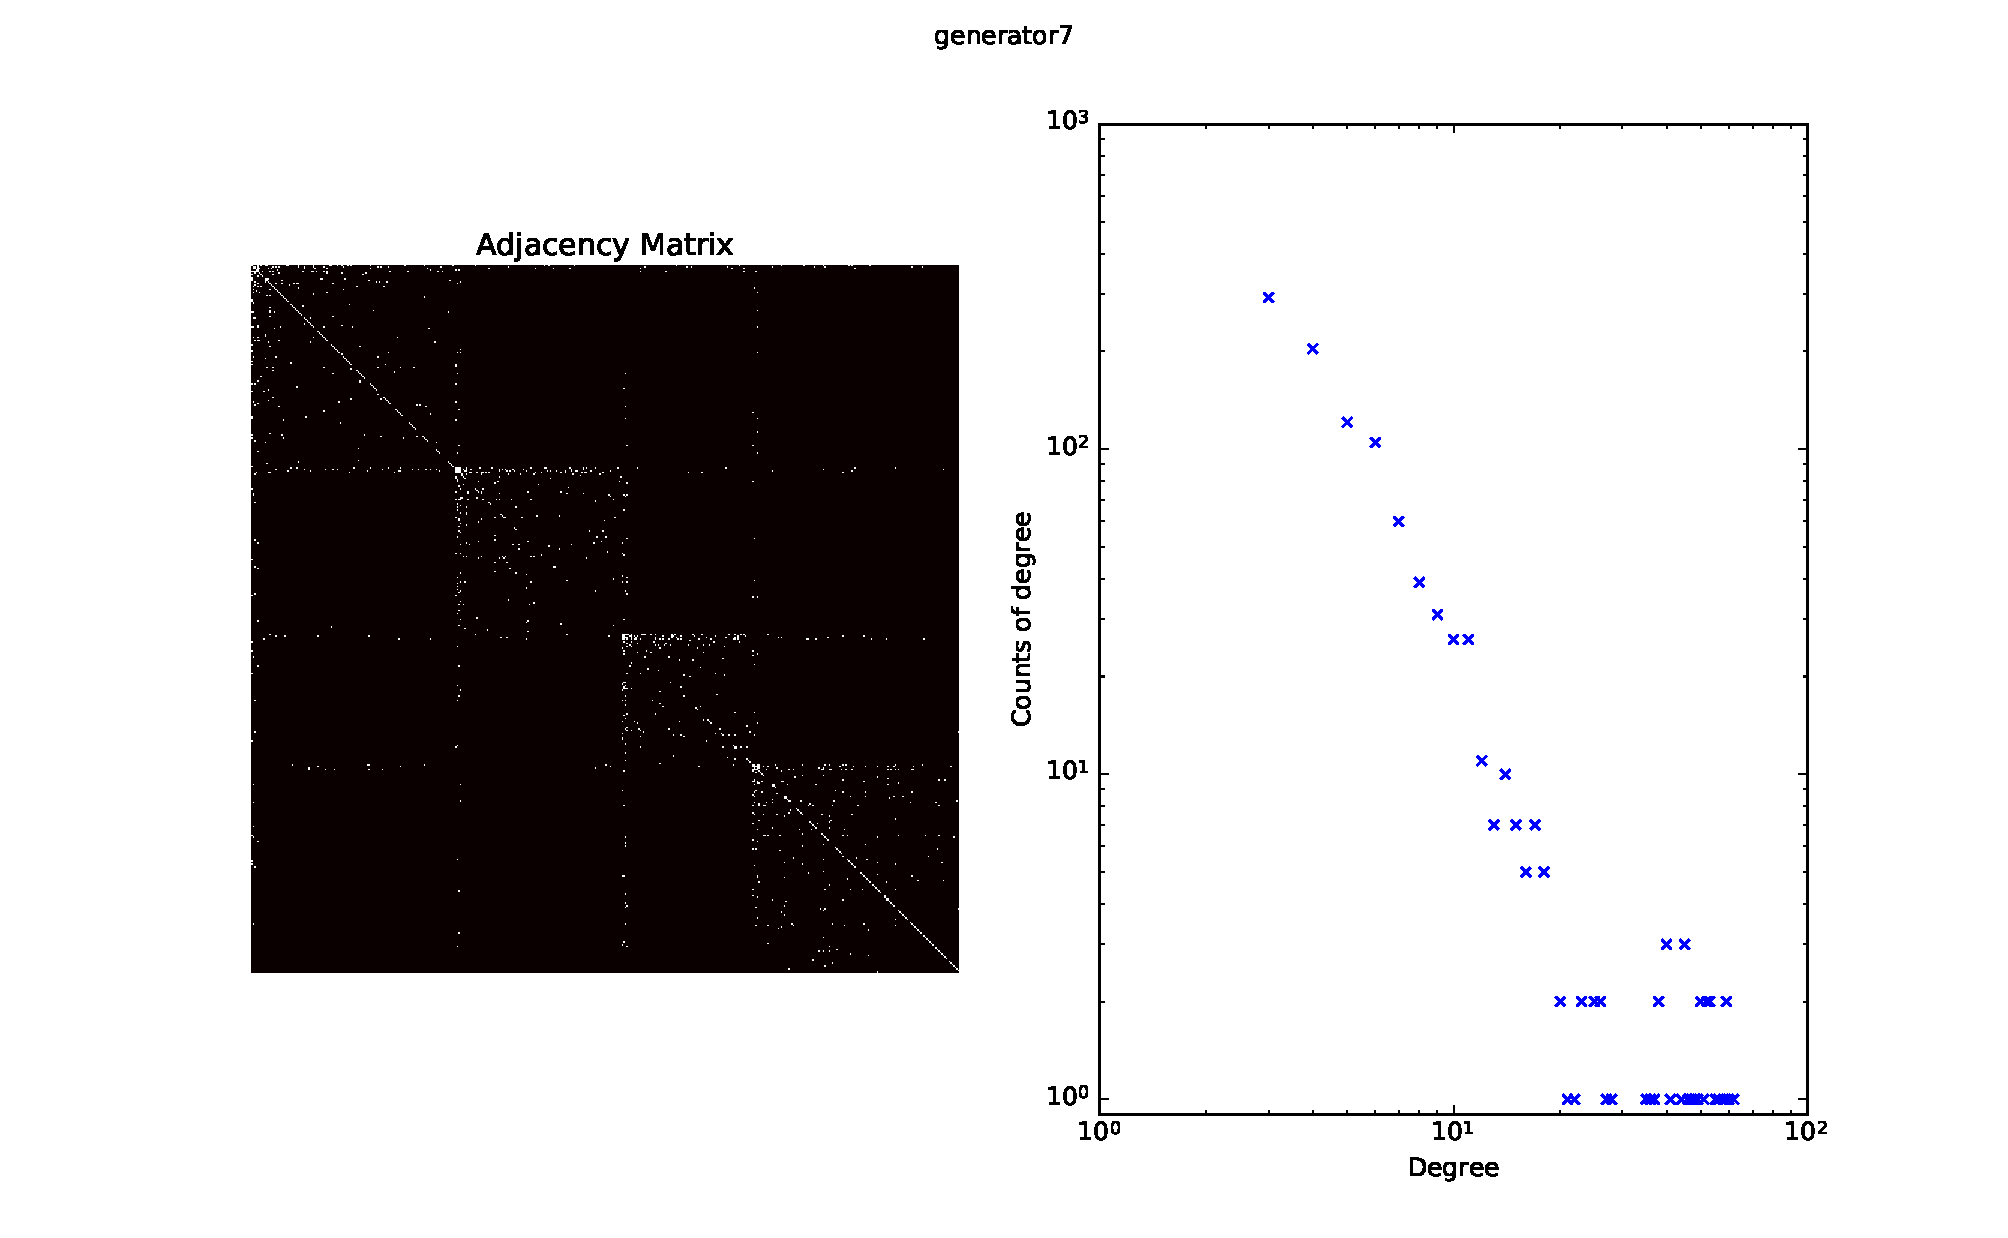
\includegraphics[scale=0.25]{img/Graph7}
	\caption{\textbf{Adjacency matrices re-ordered according to their communities.}}
	\label{fig:}
\end{figure}
\begin{figure}[h]
	\centering
	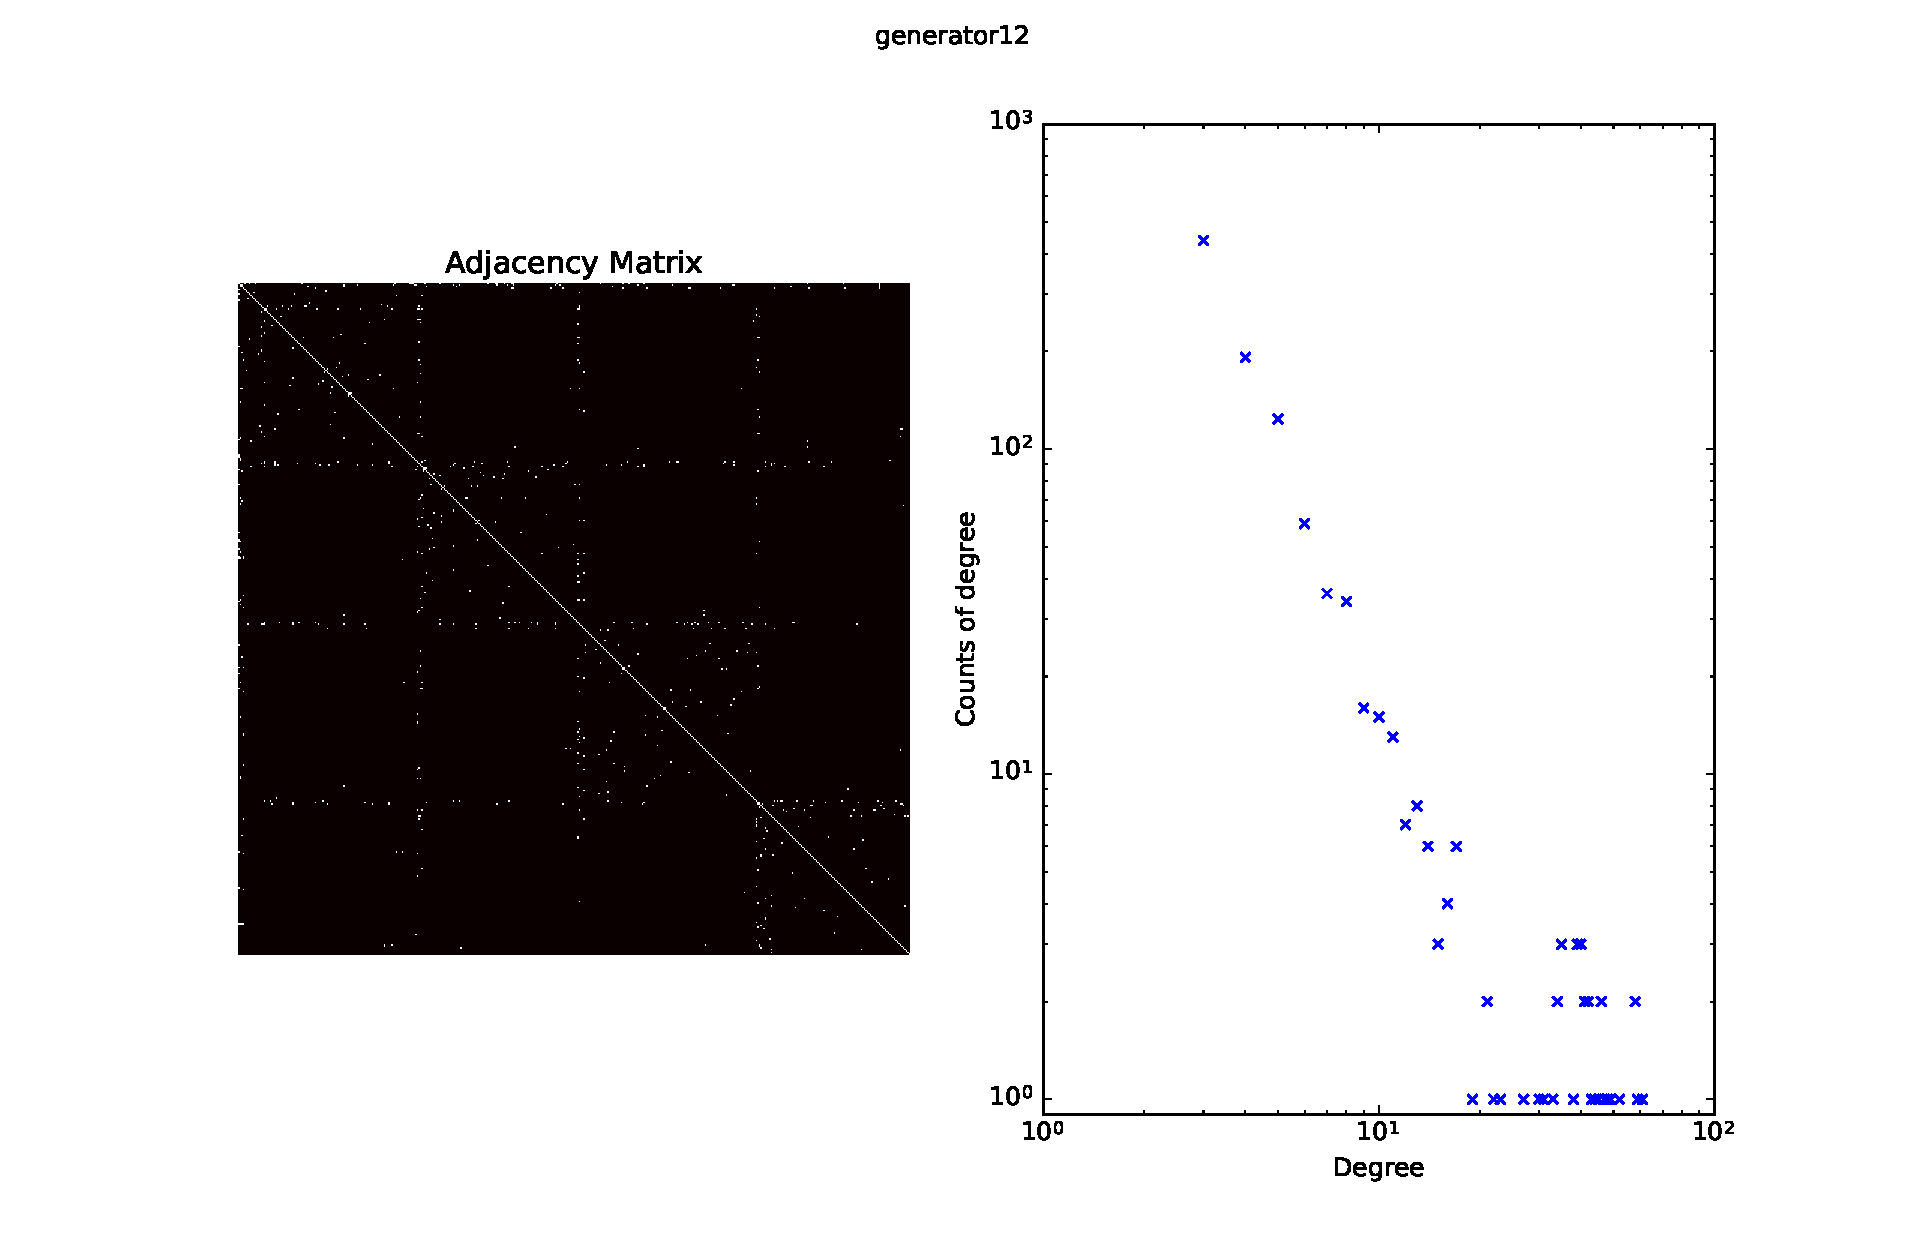
\includegraphics[scale=0.25]{img/Graph12}
	\caption{\textbf{Adjacency matrices re-ordered according to their communities.}}
	\label{fig:}
\end{figure}
\begin{figure}[h]
	\centering
	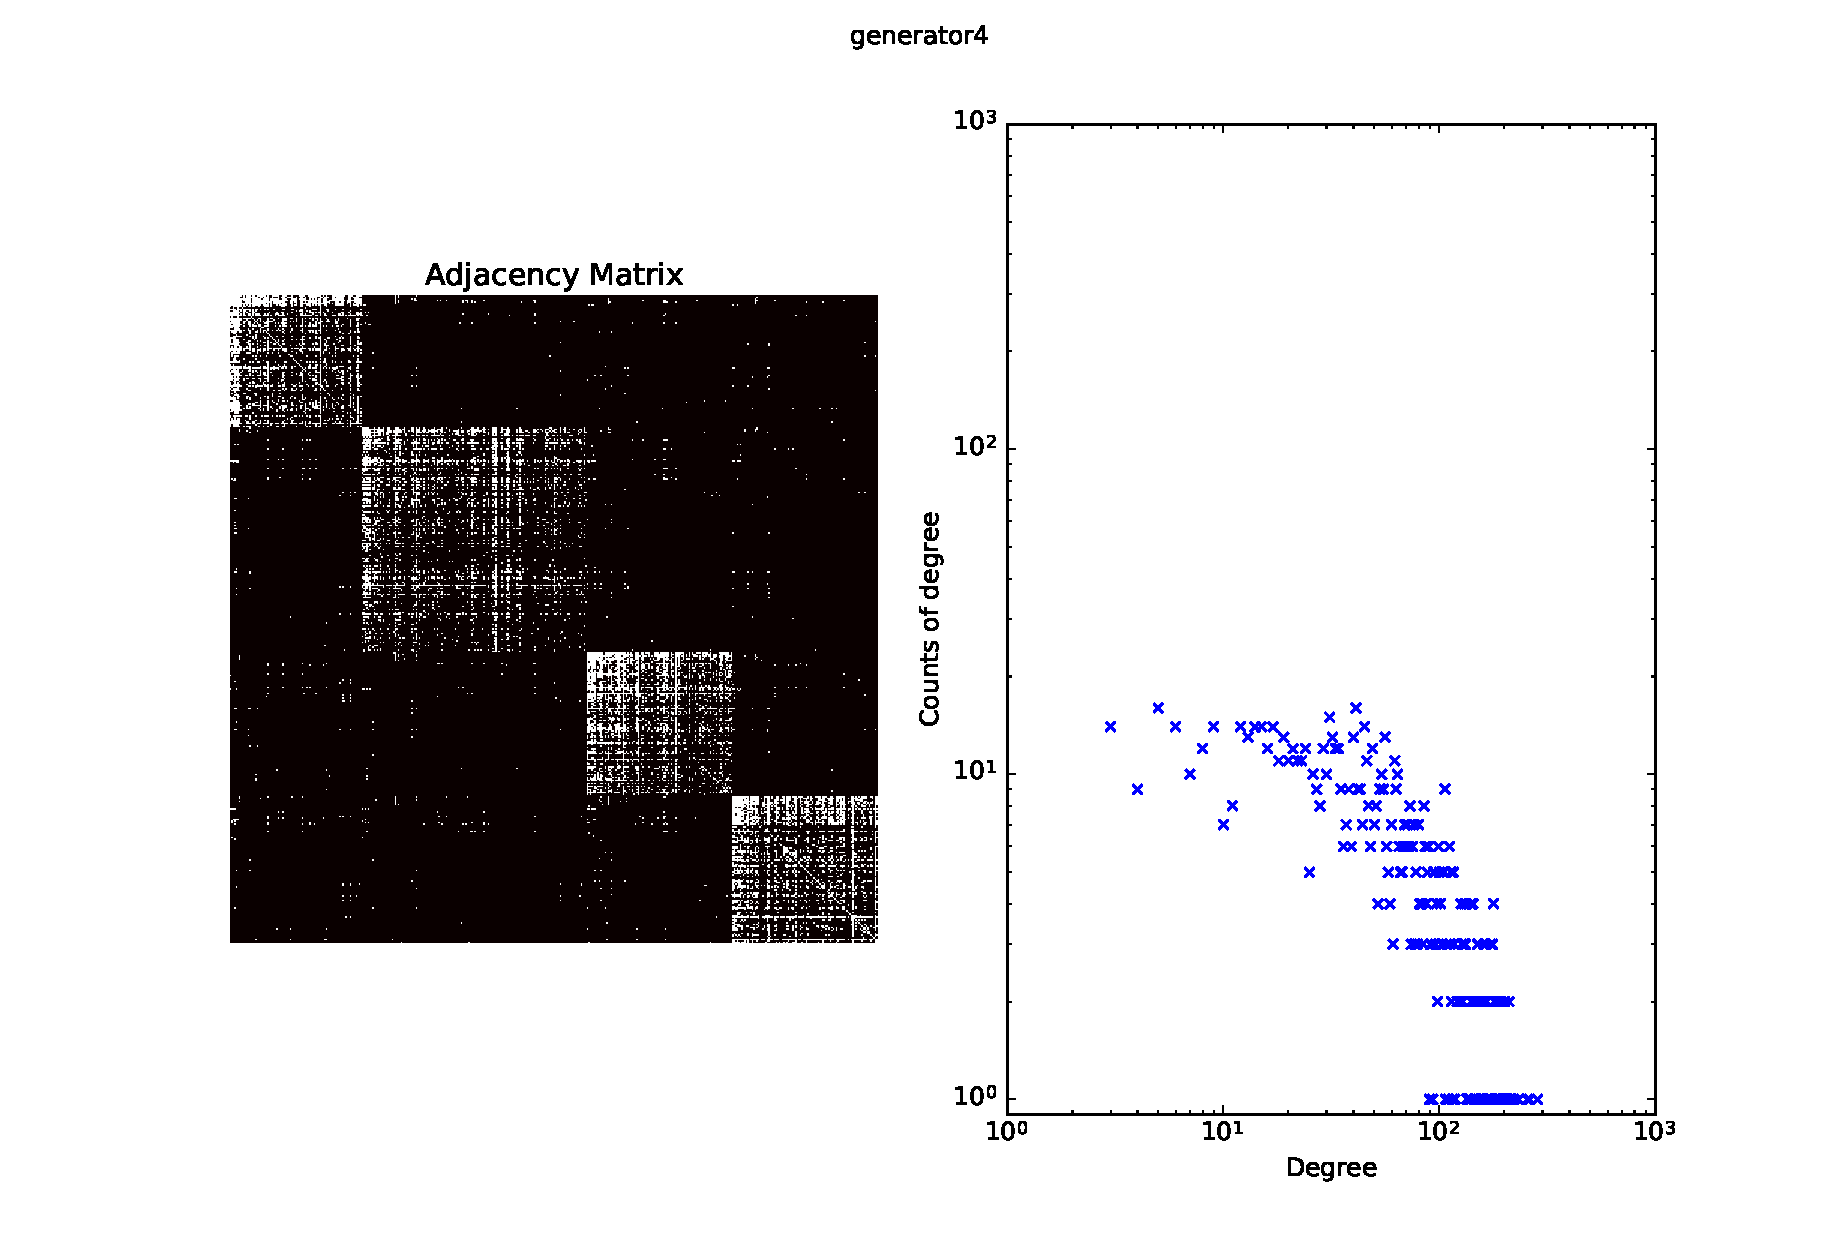
\includegraphics[scale=0.25]{img/Graph4}
	\caption{\textbf{Adjacency matrices re-ordered according to their communities.}}
	\label{fig:}
\end{figure}
\begin{figure}[h]
	\centering
	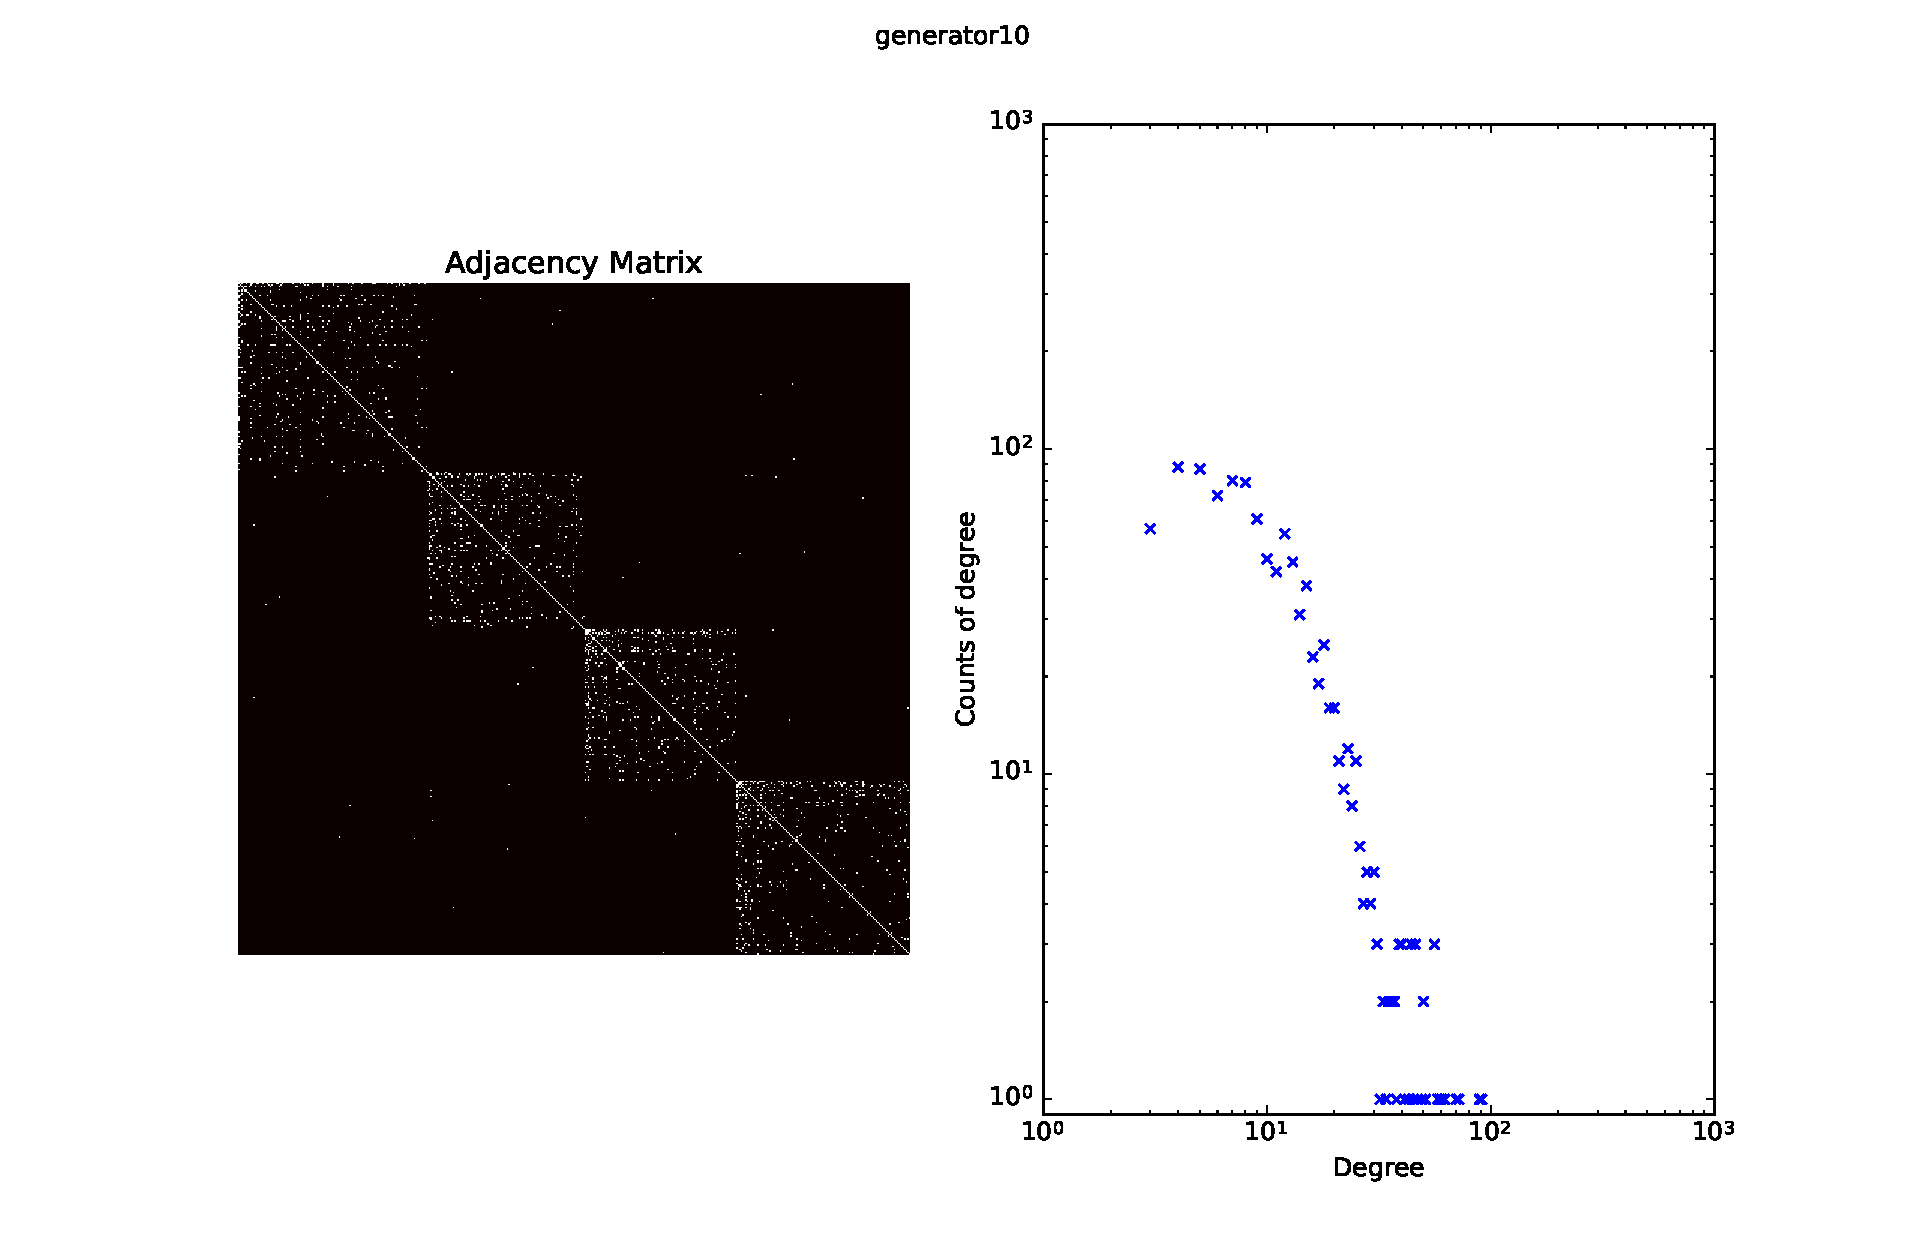
\includegraphics[scale=0.25]{img/Graph10}
	\caption{\textbf{Adjacency matrices re-ordered according to their communities.}}
	\label{fig:}
\end{figure}
%
%
%\begin{figure}[h]
%	\centering
%	
%		\minipage{0.5\textwidth}
%			\includegraphics[scale=0.4]{../figures/img/prop/gen3_com_immsb_4}
%		\endminipage
%		\minipage{0.5\textwidth}
%			\includegraphics[scale=0.4]{../figures/img/prop/gen3_com_immsb_10}
%			\endminipage
%
%	\caption{\textbf{Distribution of communities size for the class based model. The left figure correspond to number of class K=4, and the right figure correspond to K=10. The power law do not appear strongly }}
%	\label{fig:}
%\end{figure}
%


\clearpage



\begin{table*} 
\begin{minipage}[h]{0.45\linewidth}
\begin{tabular}{lrrrr}
\hline
 immsb / mask all   &        5 &       10 &       15 &       20 \\
\hline
 Graph7 b/h         & 0.989636 & 0.989939 & 0.990358 & 0.989873 \\
 Graph12 b/-h       & 0.99179  & 0.991689 & 0.991997 & 0.992259 \\
 Graph4 -b/h        & 0.886844 & 0.888035 & 0.908348 & 0.906659 \\
 Graph10 -b/-h      & 0.979057 & 0.979144 & 0.979487 & 0.979366 \\
\hline
\end{tabular}
\end{minipage}
\hspace{0.5cm}
\begin{minipage}[h]{0.45\linewidth}
\begin{tabular}{lrrrr}
\hline
 ibp / mask all   &        5 &       10 &   15 &   20 \\
\hline
 Graph7 b/h       & 0.990542 & 0.990874 &  nan &  nan \\
 Graph12 b/-h     & 0.992351 & 0.992204 &  nan &  nan \\
 Graph4 -b/h      & 0.934541 & 0.939498 &  nan &  nan \\
 Graph10 -b/-h    & 0.981383 & 0.981577 &  nan &  nan \\
\hline
\end{tabular}
\end{minipage}
\end{table*}
\begin{table*} 
	\begin{minipage}[h]{0.45\linewidth}
\begin{tabular}{lrrrr}
\hline
 immsb / mask all   &         5 &        10 &        15 &        20 \\
\hline
 Graph7 b/h         & 0.0218579 & 0.0412466 & 0.0392157 & 0.0348304 \\
 Graph12 b/-h       & 0.0346021 & 0.0280899 & 0.0360248 & 0.0494382 \\
 Graph4 -b/h        & 0.151738  & 0.159098  & 0.264185  & 0.264583  \\
 Graph10 -b/-h      & 0.0291845 & 0.0343137 & 0.0388693 & 0.028884  \\
\hline
\end{tabular}
\end{minipage}
\hspace{0.5cm}
\begin{minipage}[h]{0.45\linewidth}
\begin{tabular}{lrrrr}
\hline
 ibp / mask all   &         5 &        10 &   15 &   20 \\
\hline
 Graph7 b/h       & 0.0401146 & 0.0567951 &  nan &  nan \\
 Graph12 b/-h     & 0.0439189 & 0.0532044 &  nan &  nan \\
 Graph4 -b/h      & 0.444454  & 0.496967  &  nan &  nan \\
 Graph10 -b/-h    & 0.0743602 & 0.0910384 &  nan &  nan \\
\hline
\end{tabular}
\end{minipage}
\end{table*}
\begin{table*} 
	\begin{minipage}[h]{0.45\linewidth} 
\begin{tabular}{lrrrr}
\hline
 immsb / mask all   &         5 &        10 &        15 &        20 \\
\hline
 Graph7 b/h         & 0.0235756 & 0.0444664 & 0.0447761 & 0.0374753 \\
 Graph12 b/-h       & 0.0360577 & 0.0306373 & 0.0337995 & 0.0589812 \\
 Graph4 -b/h        & 0.192705  & 0.205694  & 0.297478  & 0.303386  \\
 Graph10 -b/-h      & 0.0341365 & 0.0369128 & 0.0436075 & 0.0337769 \\
\hline
\end{tabular}
\end{minipage}
\hspace{0.5cm}
\begin{minipage}[h]{0.45\linewidth}
\begin{tabular}{lrrrr}
\hline
 ibp / mask all   &         5 &        10 &   15 &   20 \\
\hline
 Graph7 b/h       & 0.0454545 & 0.0591966 &  nan &  nan \\
 Graph12 b/-h     & 0.0544693 & 0.0537897 &  nan &  nan \\
 Graph4 -b/h      & 0.462571  & 0.490113  &  nan &  nan \\
 Graph10 -b/-h    & 0.0784913 & 0.09826   &  nan &  nan \\
\hline
\end{tabular}
\end{minipage}
\end{table*}


%\hline



\begin{table*} 
	\begin{minipage}[h]{0.45\linewidth} 
\begin{tabular}{lrrrr}
\hline
 immsb / mask all   &   global &   precision &    rappel &   K-\ensuremath{>} \\
\hline
 Graph7b/h          & 0.989636 &   0.0218579 & 0.0235756 &     5 \\
 Graph12 b/-h       & 0.99179  &   0.0346021 & 0.0360577 &     5 \\
 Graph4 -b/h        & 0.886844 &   0.151738  & 0.192705  &     5 \\
 Graph10 -b/-h      & 0.979057 &   0.0291845 & 0.0341365 &     5 \\
\hline
\end{tabular}
\end{minipage}
\hspace{0.5cm}
\begin{minipage}[h]{0.45\linewidth}
\begin{tabular}{lrrrr}
\hline
 ibp / mask all   &   global &   precision &    rappel &   K-\ensuremath{>} \\
\hline
 Graph7b/h        & 0.990542 &   0.0401146 & 0.0454545 &    21 \\
 Graph12 b/-h     & 0.992351 &   0.0439189 & 0.0544693 &    19 \\
 Graph4 -b/h      & 0.934541 &   0.444454  & 0.462571  &     8 \\
 Graph10 -b/-h    & 0.981383 &   0.0743602 & 0.0784913 &     8 \\
\hline
\end{tabular}
\end{minipage}
\end{table*}


\begin{table*} 
	\begin{minipage}[h]{0.45\linewidth} 
\begin{tabular}{lrrrr}
\hline
 immsb / mask all   &   global &   precision &    rappel &   K-\ensuremath{>} \\
\hline
 Graph7b/h          & 0.989939 &   0.0412466 & 0.0444664 &    10 \\
 Graph12 b/-h       & 0.991689 &   0.0280899 & 0.0306373 &    10 \\
 Graph4 -b/h        & 0.888035 &   0.159098  & 0.205694  &    10 \\
 Graph10 -b/-h      & 0.979144 &   0.0343137 & 0.0369128 &    10 \\
\hline
\end{tabular}
\end{minipage}
\hspace{0.5cm}
\begin{minipage}[h]{0.45\linewidth}
\begin{tabular}{lrrrr}
\hline
 ibp / mask all   &   global &   precision &    rappel &   K-\ensuremath{>} \\
\hline
 Graph7b/h        & 0.990874 &   0.0567951 & 0.0591966 &    16 \\
 Graph12 b/-h     & 0.992204 &   0.0532044 & 0.0537897 &    13 \\
 Graph4 -b/h      & 0.939498 &   0.496967  & 0.490113  &    10 \\
 Graph10 -b/-h    & 0.981577 &   0.0910384 & 0.09826   &    11 \\
\hline
\end{tabular}
\end{minipage}
\end{table*}


\begin{table*} 
	\begin{minipage}[h]{0.45\linewidth} 
\begin{tabular}{lrrrr}
\hline
 immsb / mask all   &   global &   precision &    rappel &   K-\ensuremath{>} \\
\hline
 Graph7b/h          & 0.990358 &   0.0392157 & 0.0447761 &    15 \\
 Graph12 b/-h       & 0.991997 &   0.0360248 & 0.0337995 &    15 \\
 Graph4 -b/h        & 0.908348 &   0.264185  & 0.297478  &    15 \\
 Graph10 -b/-h      & 0.979487 &   0.0388693 & 0.0436075 &    15 \\
\hline
\end{tabular}
\end{minipage}
\hspace{0.5cm}
\begin{minipage}[h]{0.45\linewidth}
\begin{tabular}{lrrrr}
\hline
 ibp / mask all   &   global &   precision &   rappel &   K-\ensuremath{>} \\
\hline
 Graph7b/h        &      nan &         nan &      nan &   nan \\
 Graph12 b/-h     &      nan &         nan &      nan &   nan \\
 Graph4 -b/h      &      nan &         nan &      nan &   nan \\
 Graph10 -b/-h    &      nan &         nan &      nan &   nan \\
\hline
\end{tabular}
\end{minipage}
\end{table*}


\begin{table*} 
	\begin{minipage}[h]{0.45\linewidth} 
\begin{tabular}{lrrrr}
\hline
 immsb / mask all   &   global &   precision &    rappel &   K-\ensuremath{>} \\
\hline
 Graph7b/h          & 0.989873 &   0.0348304 & 0.0374753 &    20 \\
 Graph12 b/-h       & 0.992259 &   0.0494382 & 0.0589812 &    20 \\
 Graph4 -b/h        & 0.906659 &   0.264583  & 0.303386  &    20 \\
 Graph10 -b/-h      & 0.979366 &   0.028884  & 0.0337769 &    20 \\
\hline
\end{tabular}
\end{minipage}
\hspace{0.5cm}
\begin{minipage}[h]{0.45\linewidth}
\begin{tabular}{lrrrr}
\hline
 ibp / mask all   &   global &   precision &   rappel &   K-\ensuremath{>} \\
\hline
 Graph7b/h        &      nan &         nan &      nan &   nan \\
 Graph12 b/-h     &      nan &         nan &      nan &   nan \\
 Graph4 -b/h      &      nan &         nan &      nan &   nan \\
 Graph10 -b/-h    &      nan &         nan &      nan &   nan \\
\hline
\end{tabular}
\end{minipage}
\end{table*}





\clearpage
